\chapter{User documentation}
\label{chap:user_documentation}

In this chapter we show the user interface of our web application and describe how all our main LLM assistant features are used through the user interface.


\section{Suggestions of classes, attributes and associations}

The domain modeling process usually starts by providing a domain description. We support domain descriptions only in the English language. For trying out the application the \textit{data catalog}\footnote{\url{https://github.com/dataspecer/domain-modeling-benchmark/blob/main/front-end\%20evaluation\%20domains/data\%20catalog/domain-description-01.txt}} or \textit{gaming}\footnote{\url{https://github.com/dataspecer/domain-modeling-benchmark/blob/main/front-end\%20evaluation\%20domains/gaming/domain-description-01.txt}} domain description can be used.

The domain description can be inserted in the text box on the topbar as shown in the picture \ref{fig:domain-description-text-box}:

\begin{figure}[!h]
    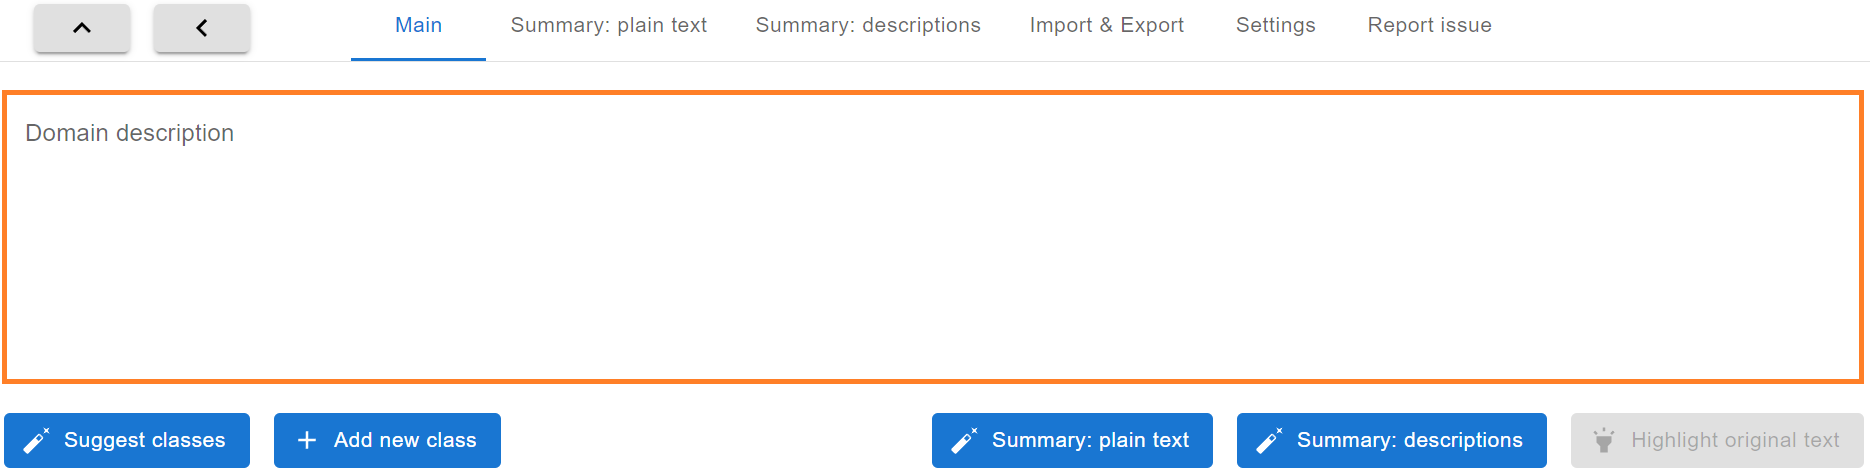
\includegraphics[scale=0.36]{../docs/images/frontend/insert-domain-description.png}
    \caption{\centering Text box for inserting the domain description}
    \label{fig:domain-description-text-box}
\end{figure}

When the domain description is not provided the assistant suggests anything it considers reasonable. In this case, it is better to start modeling by adding a class manually with the \textit{Add new class} button as shown in the picture \ref{fig:add_new_class}.

\begin{figure}[!h]
    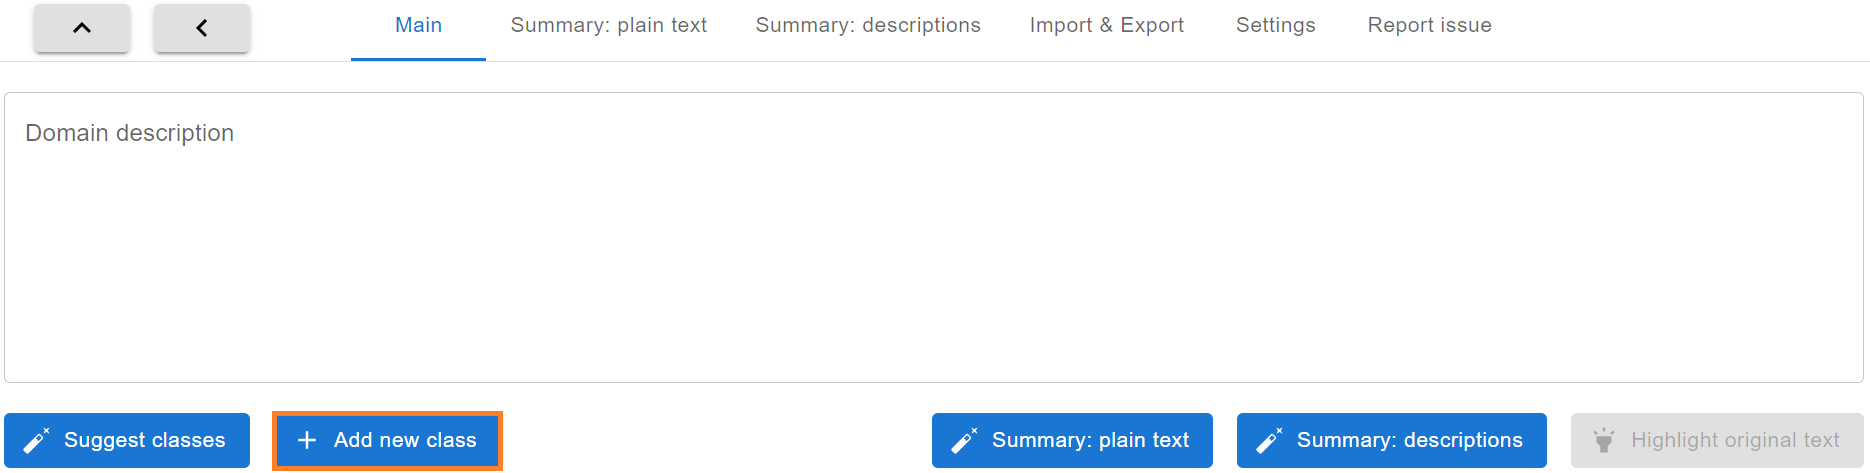
\includegraphics[scale=0.36]{../docs/images/frontend/add-new-class-manually.png}
    \caption{\centering The \textit{Add new class} button for manually adding classes into the domain model}
    \label{fig:add_new_class}
\end{figure}

For suggesting classes by the assistant the \textit{Suggest classes} button can be used as shown in the picture \ref{fig:suggest_classes}.

\begin{figure}[!h]
    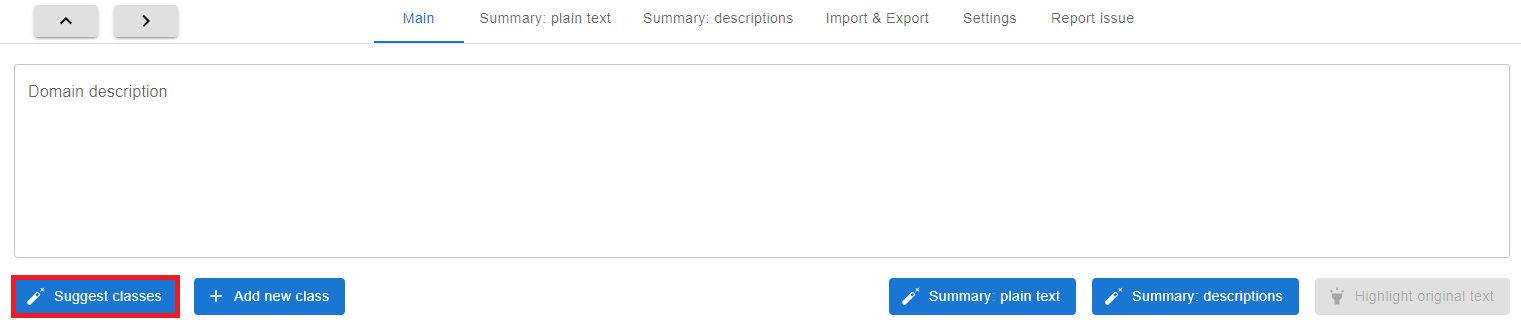
\includegraphics[scale=0.36]{../docs/images/frontend/suggest-classes.png}
    \caption{\centering The \textit{Suggest classes} button for suggesting classes by the assistant}
    \label{fig:suggest_classes}
\end{figure}

To have attributes and associations suggested by the assistant, first, create a class and then hover the mouse over this class, click on the three dots on the right side, and select either the \textit{Suggest attributes} or \textit{Suggest associations} button accordingly as shown in the picture \ref{fig:suggest_attributes}

\begin{figure}[!h]
    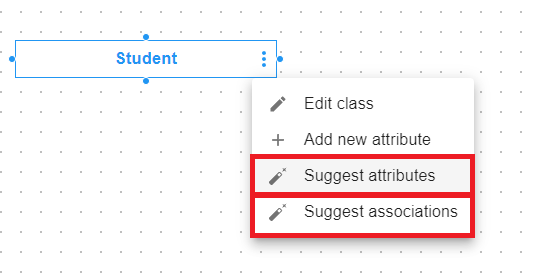
\includegraphics[scale=0.45]{../docs/images/frontend/suggest-attributes.png}
    \caption{\centering The \textit{Suggest attributed} and \textit{Suggest associations} button for suggesting attributed and associations by the assistant}
    \label{fig:suggest_attributes}
\end{figure}

The generated suggestions are shown in the sidebar on the right side of the application. The picture \ref{fig:suggested_classes} shows an example of 5 generated suggestions that were generated by clicking on the \textit{Suggest classes} button without providing a domain description.

\begin{figure}[!h]
    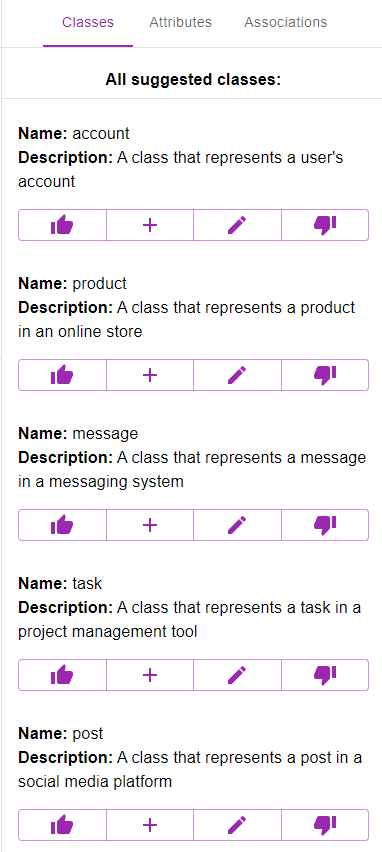
\includegraphics[scale=0.45]{../docs/images/frontend/suggested-classes.png} \\
    \begin{itemize}
    \item the \textit{plus} button can be used to add the corresponding suggestion to the domain model
    \item the \textit{edit} button can be used to first edit the corresponding suggestion and then add it to the domain model
    \item the \textit{like} or \textit{dislike} button can be used to rate the corresponding suggestion
    \end{itemize}
    \caption{\centering Example of generated suggestion for classes without provided domain description}
    \label{fig:suggested_classes}
\end{figure}

When editing an attribute it can be changed into an association as discussed in the section \ref{sec:attributes_and_associations_conversion} and vice versa. This is shown in the picture \ref{fig:change_to_association}.

\begin{figure}[!h]
    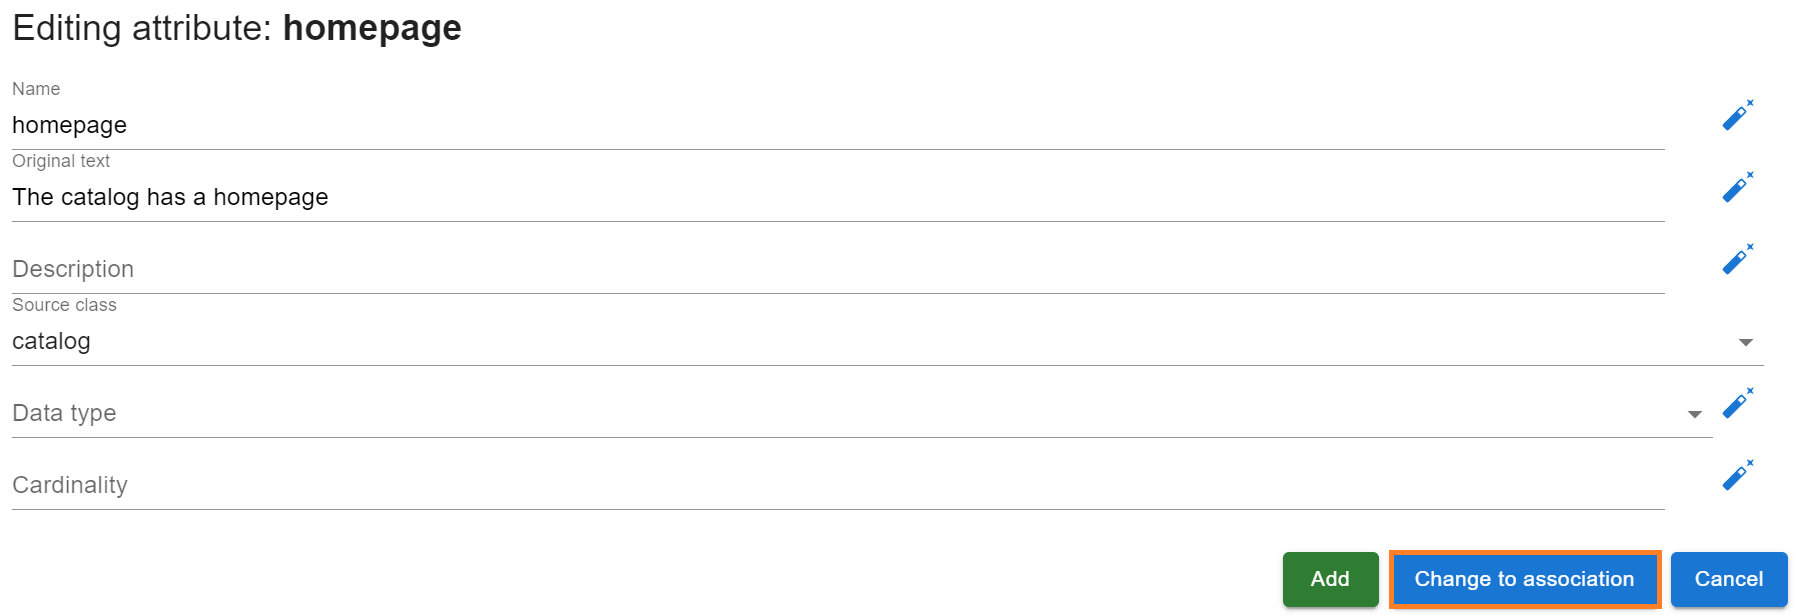
\includegraphics[scale=0.36]{../docs/images/frontend/change-to-association.png}
    \caption{\centering The \textit{Change to association} button used for converting an attribute into an association}
    \label{fig:change_to_association}
\end{figure}

If the domain description is provided then for each suggestion is also available the \textit{highlight} button that for attributes and associations shows in which part of the domain description the assistant found the corresponding suggestion as discussed in the section \ref{sec:context_highlighting}. For example, the highlighted original text for the attribute \textit{homepage} of the class \textit{catalog} is shown in the picture \ref{fig:highlight_original_text}

\begin{figure}[!h]
    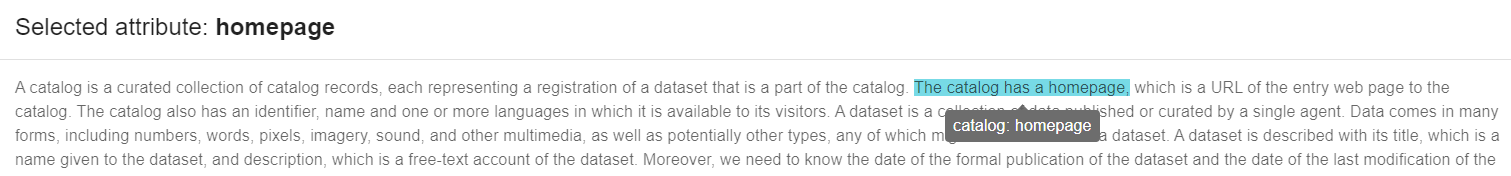
\includegraphics[scale=0.36]{../docs/images/frontend/highlight-original-text.png}
    \caption{\centering Highlighted original text for the attribute \textit{homepage} of the class \textit{catalog}}
    \label{fig:highlight_original_text}
\end{figure}

For suggesting associations in between two classes an edge can be dragged between two nodes as shown in the picture \ref{fig:edge_drag}

\begin{figure}[!h]
    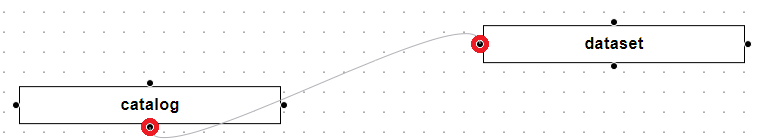
\includegraphics[scale=0.4]{../docs/images/frontend/edge-drag.png}
    \caption{\centering Demonstration of connecting two classes with an edge}
    \label{fig:edge_drag}
\end{figure}

This opens a dialogue where by clicking on the \textit{Suggest associations} button as shown in the picture \ref{fig:suggest_associations_2}, the assistant suggests corresponding associations between those two classes.

\begin{figure}[!h]
    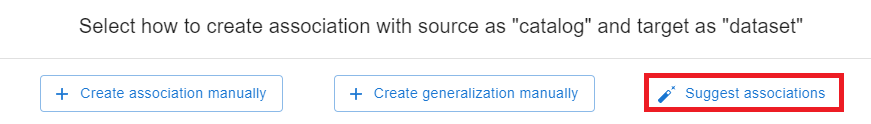
\includegraphics[scale=0.4]{../docs/images/frontend/suggest-associations-2.png}
    \caption{\centering The \textit{Suggest associations} button used for suggesting associations between two classes}
    \label{fig:suggest_associations_2}
\end{figure}

Note that an edge can be dragged only between the handles (the ``black dots'') of the nodes. When the mouse is hovered over any node, the handles display either ``\textit{s}'' or ``\textit{t}'' as shown in the picture \ref{fig:handles}.

\begin{figure}[!h]
    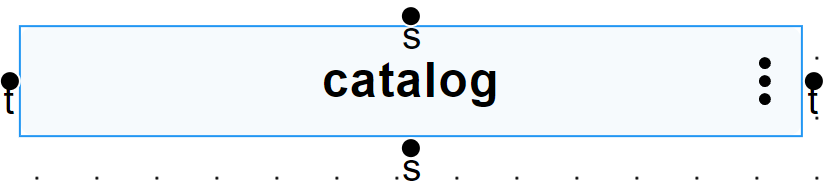
\includegraphics[scale=0.5]{../docs/images/frontend/handles.png}
    \caption{\centering The ``\textit{s}'' (source) and ``\textit{t}'' (target) handles when the mouse hovers over a class}
    \label{fig:handles}
\end{figure}

The ``\textit{s}'' stands for the source class and ``\textit{t}'' stands for the target class of the possible association. An edge can be dragged either from ``\textit{s}'' to ``\textit{t}'' or from ``\textit{t}'' to ``\textit{s}''.

When editing any element the \textit{magic wand} button can be used on the right side to let the assistant suggest the corresponding field as shown in the picture \ref{fig:suggest_single_field}.

\begin{figure}[!h]
    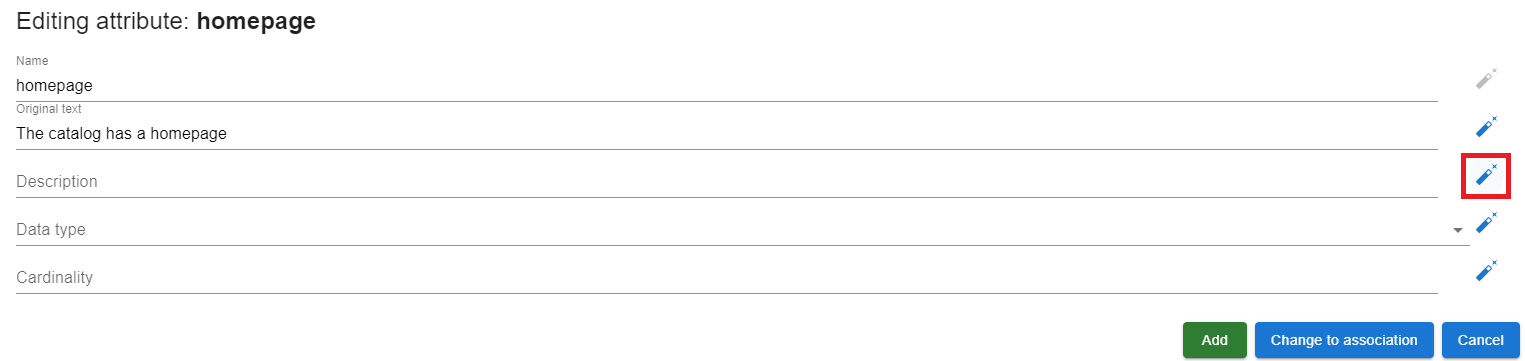
\includegraphics[scale=0.35]{../docs/images/frontend/suggest-single-field.png}
    \caption{\centering The \textit{magic wand} button for suggesting a description for the attribute \textit{homepage}}
    \label{fig:suggest_single_field}
\end{figure}

For example, the suggested description for the attribute \textit{homepage} of the class \textit{catalog} is shown in the picture \ref{fig:suggested_single_field}.

\begin{figure}[!h]
    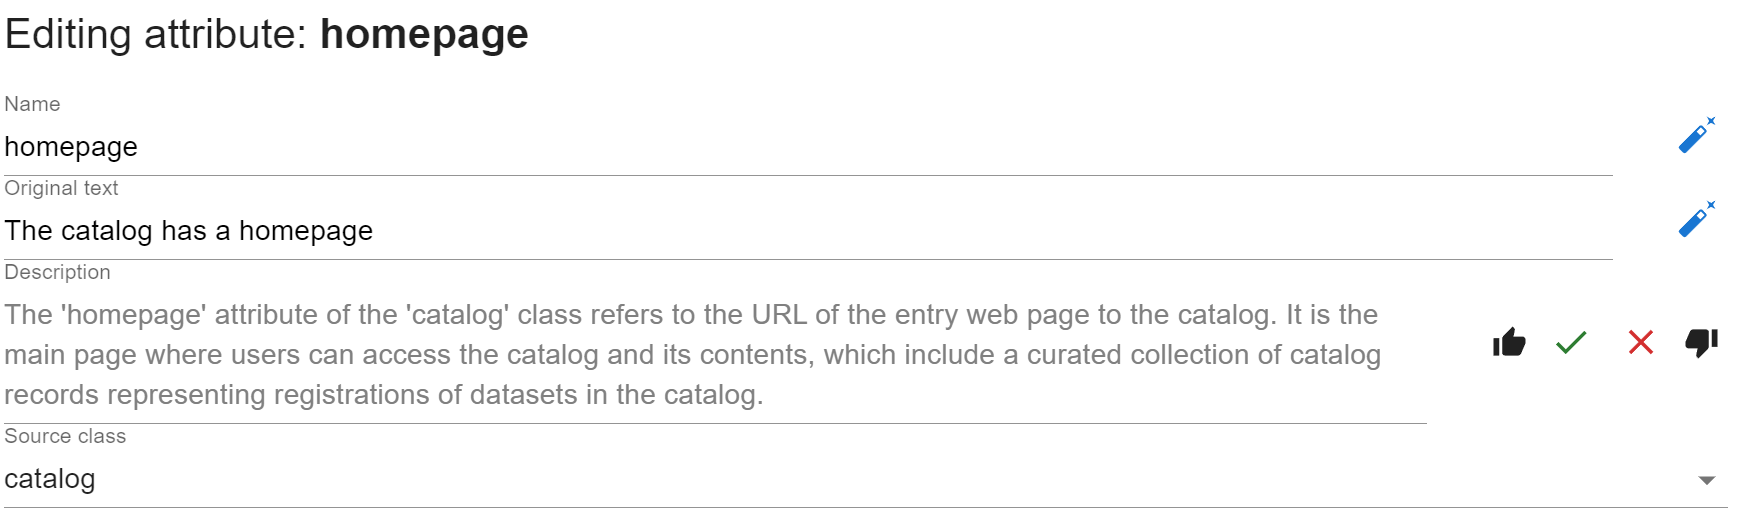
\includegraphics[scale=0.35]{../docs/images/frontend/suggested-single-field.png}
    \caption{\centering Example of suggested description for the attribute \textit{homepage}}
    \label{fig:suggested_single_field}
\end{figure}

The suggestion can be accepted or rejected with the buttons on the right side.


\section{Summary of the domain model}

The assistant can summarize any selected part of the domain model. The selected domain elements are visually represented by the blue color. The easiest way to select some parts of the domain model is by creating a selection area with the mouse by holding the shift and the left mouse button as shown in the picture \ref{fig:selection}.

\begin{figure}[!h]
    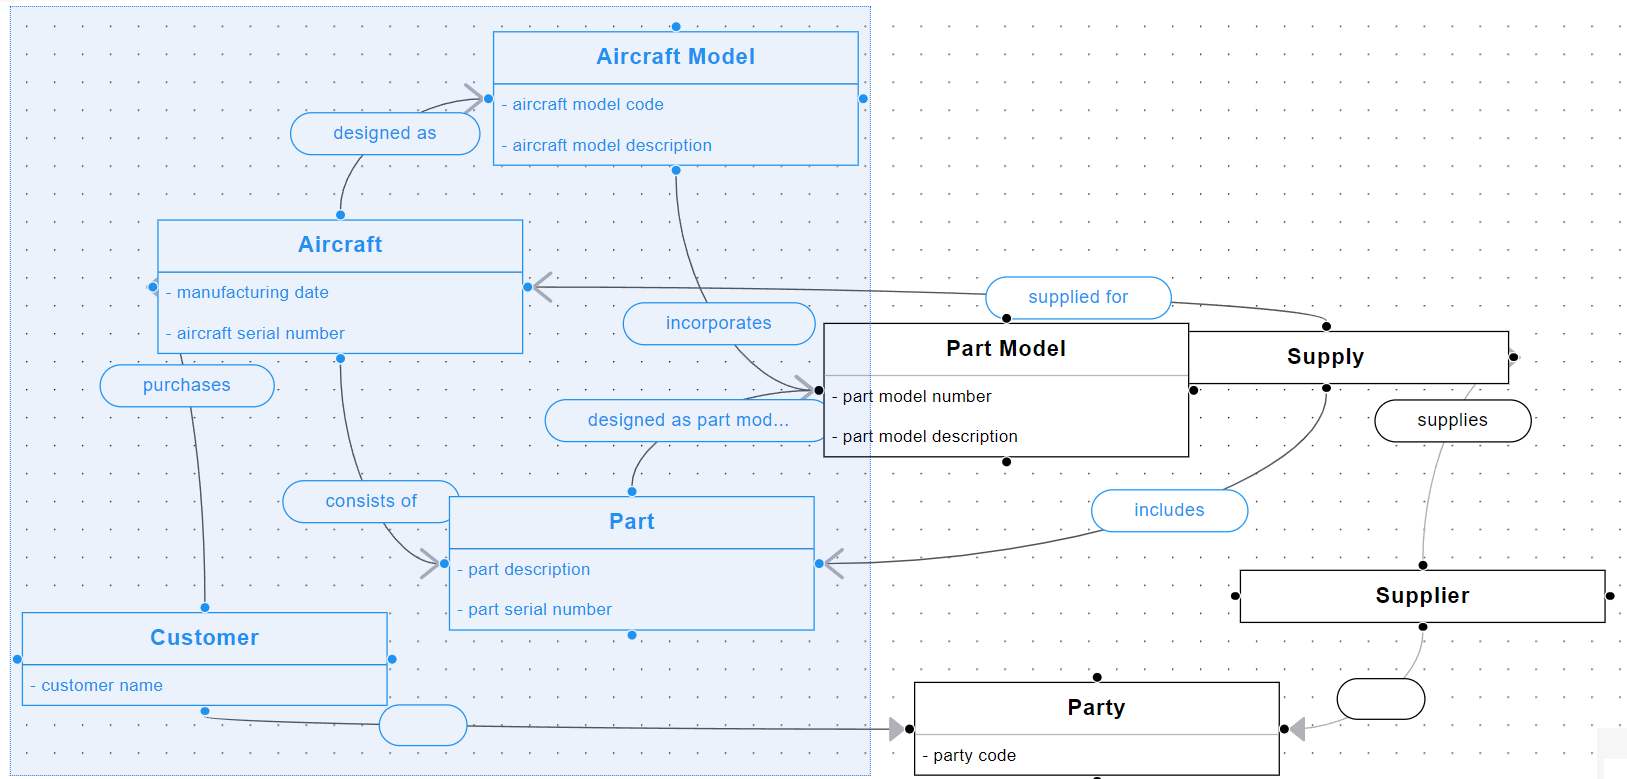
\includegraphics[scale=0.4]{../docs/images/frontend/selection.png}
    \caption{\centering Example of selecting part of the domain model with the ``\textit{select area}'' utility}
    \label{fig:selection}
\end{figure}

When some part of the domain model is selected, the assistant can summarize this part either in an unstructured plain text by clicking on the topbar on the button \textit{Summary: plain text} or in structured descriptions by clicking on the button \textit{Summary: descriptions}. These buttons are shown in the picture \ref{fig:summary_buttons}.

\begin{figure}[!h]
    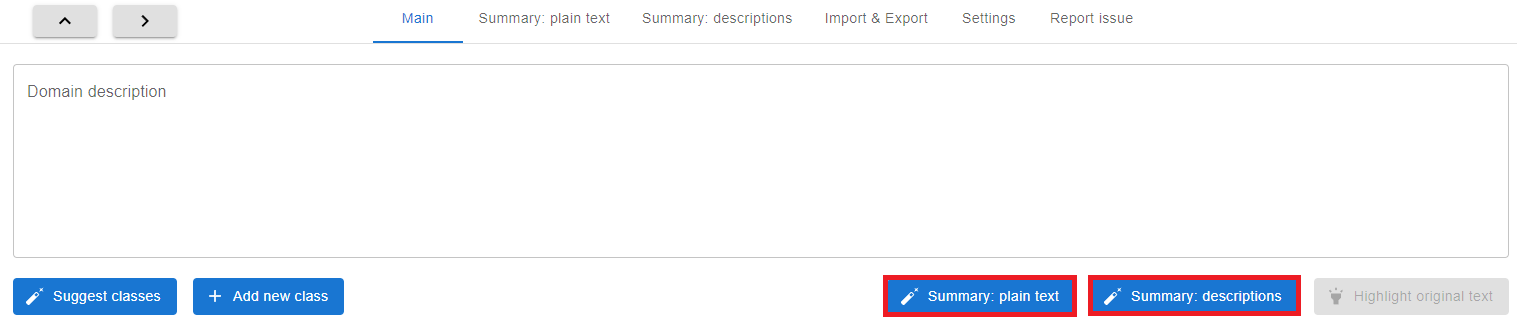
\includegraphics[scale=0.35]{../docs/images/frontend/summary-buttons.png}
    \caption{\centering The \textit{Summary: plain text} button and \textit{Summary: descriptions} button for generating summary for the selected part of the domain model}
    \label{fig:summary_buttons}
\end{figure}

For example, consider the selected part of the domain model as shown in the picture \ref{fig:selection_aircraft}.

\begin{figure}[!h]
    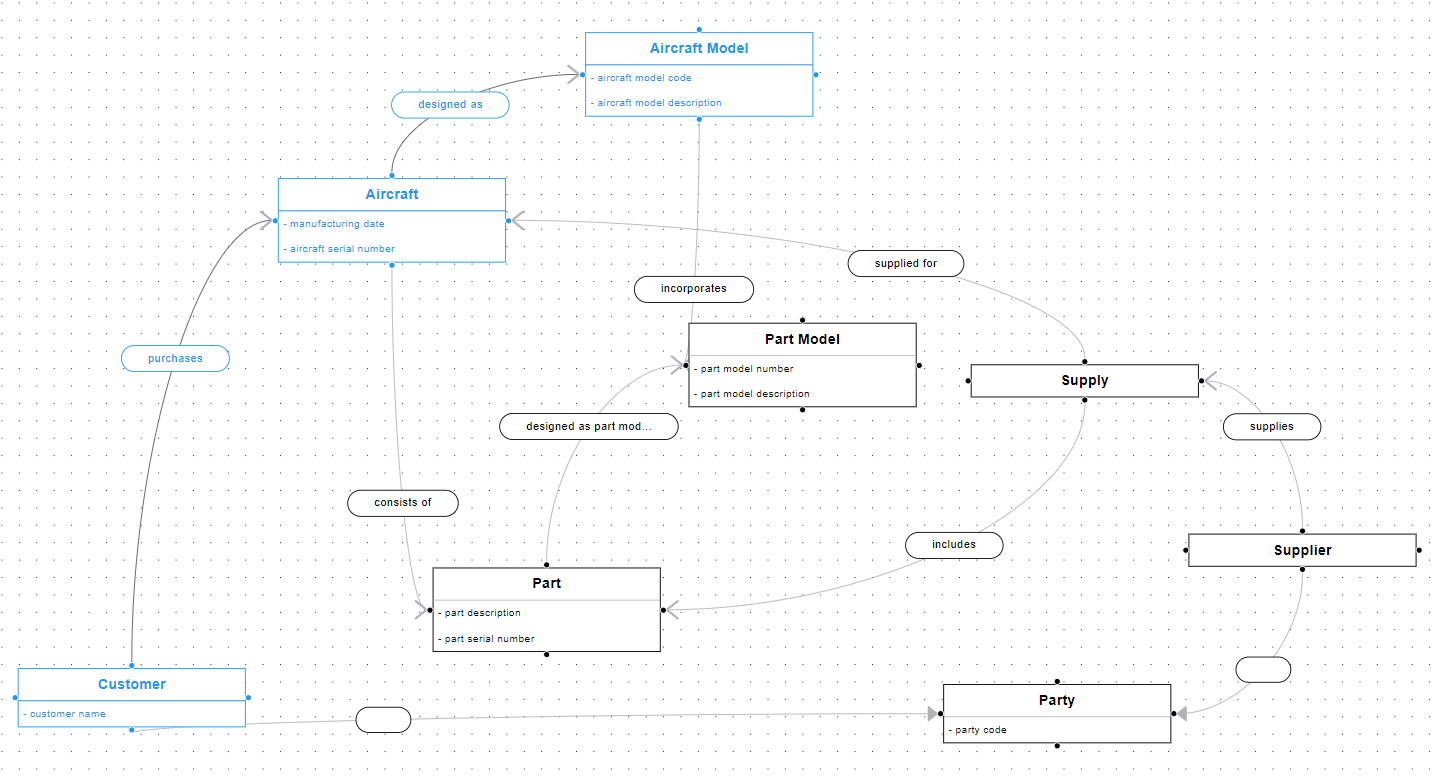
\includegraphics[scale=0.38]{../docs/images/frontend/selection-aircraft.png}
    \caption{\centering Example of some selected domain elements of domain model for aircraft manufacturing}
    \label{fig:selection_aircraft}
\end{figure}

Then the example of the output generated by the \textit{Summary: plain text} button is shown in the picture \ref{fig:summary_plain_text} and the example of the output generated by the \textit{Summary: descriptions} button is shown in the picture \ref{fig:summary_description}.

\begin{figure}[!h]
    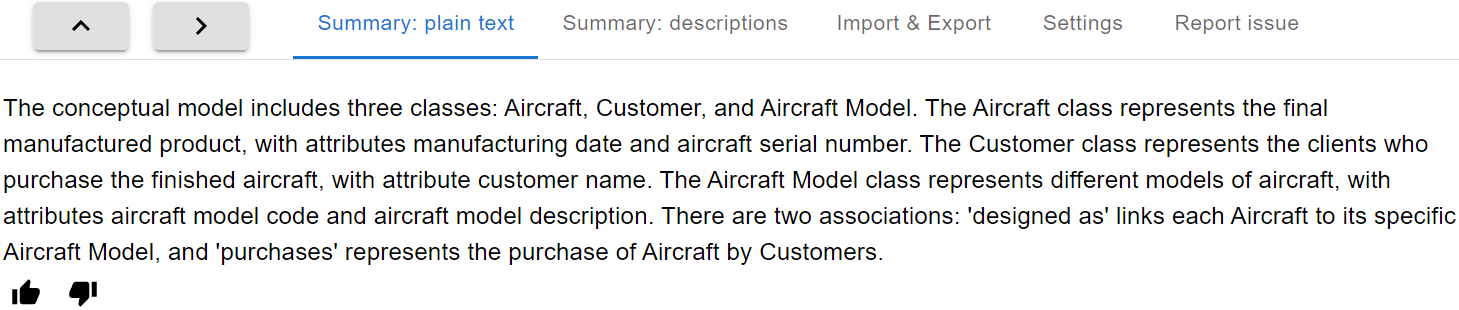
\includegraphics[scale=0.295]{../docs/images/frontend/summary-plain-text.png}
    \caption{\centering Example of the generated summary when clicking on the \textit{Summary: plain text} button.}
    \label{fig:summary_plain_text}
\end{figure}

\begin{figure}[!h]
    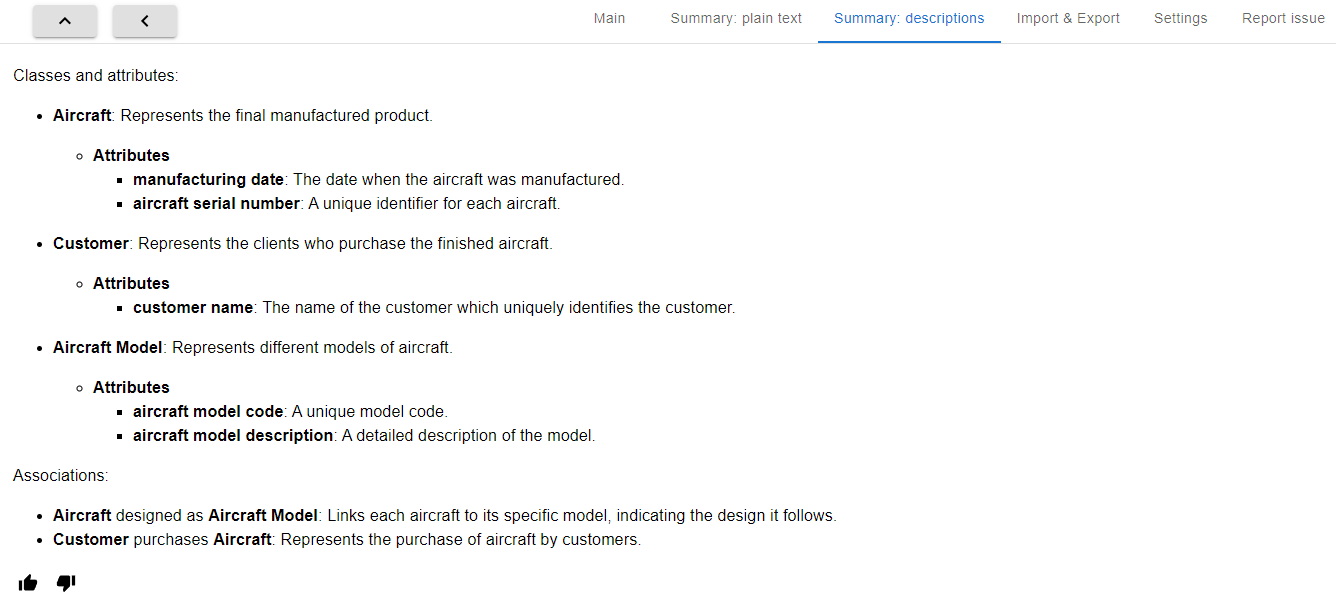
\includegraphics[scale=0.41]{../docs/images/frontend/summary-descriptions.png}
    \caption{\centering Example of the generated summary when clicking on the \textit{Summary: descriptions} button.}
    \label{fig:summary_description}
\end{figure}

Note that the assistant ignores the domain description when generating the summary.


\section{Highlighting which parts are modeled}

When a domain description is provided and when creating a domain model with the help of the assistant each suggested element contains also the original text. When some part of the domain model is selected all these original texts can be highlighted in the domain description using the \textit{Highlight original text} button on the topbar as shown in the picture \ref{fig:highlight_original_text_button}.

\begin{figure}[!h]
    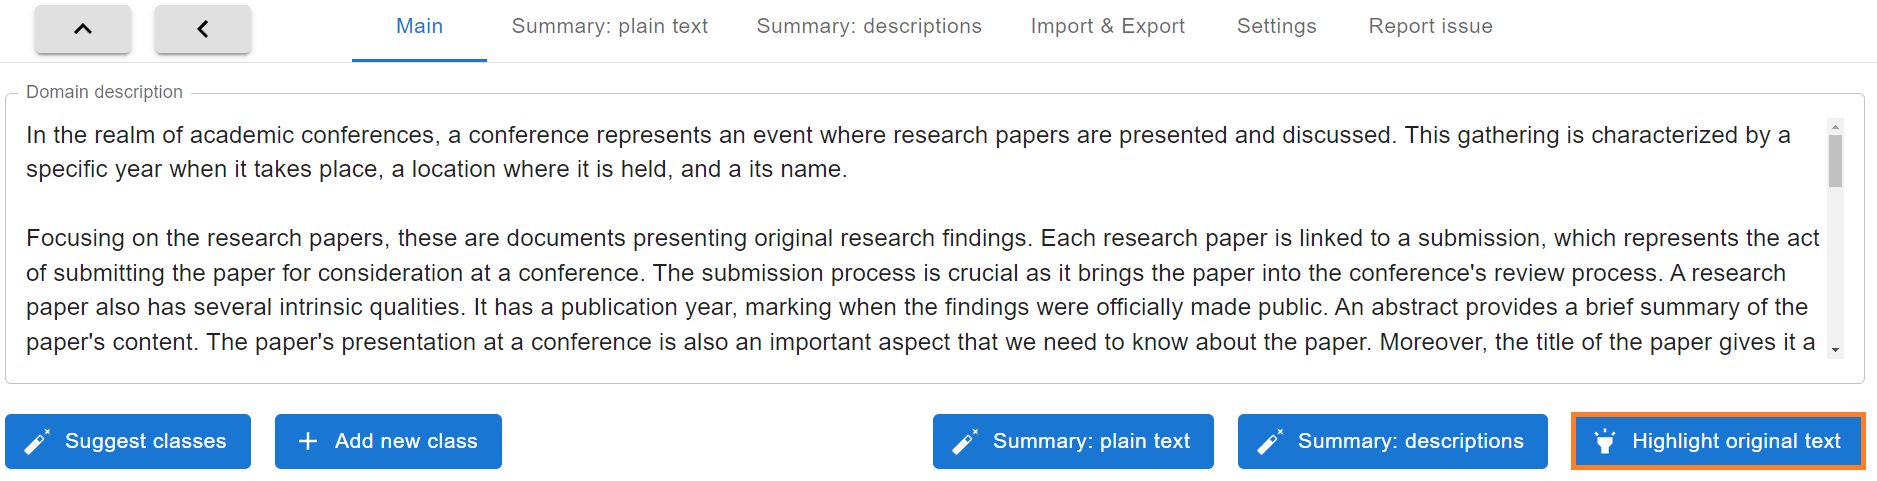
\includegraphics[scale=0.36]{../docs/images/frontend/highlight-original-text-button.png}
    \caption{\centering The \textit{Highlight original text} button for highlighting the original text in the domain description for the selected part of the domain model}
    \label{fig:highlight_original_text_button}
\end{figure}

For example, for a domain description about conference papers and the class \textit{conference} with the attributes \textit{year}, \textit{location}, \textit{name} as shown in the picture \ref{fig:class_example}.

\begin{figure}[!h]
    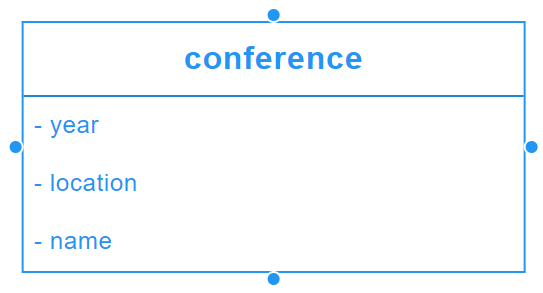
\includegraphics[scale=0.3]{../docs/images/frontend/class-example.png}
    \caption{\centering Example of class \textit{conference} with the attributes \textit{year}, \textit{location} and \textit{name}}
    \label{fig:class_example}
\end{figure}

The picture \ref{fig:highlight_all_example} shows one of the possible outputs of the \textit{Highlight original text} button.

\begin{figure}[!h]
    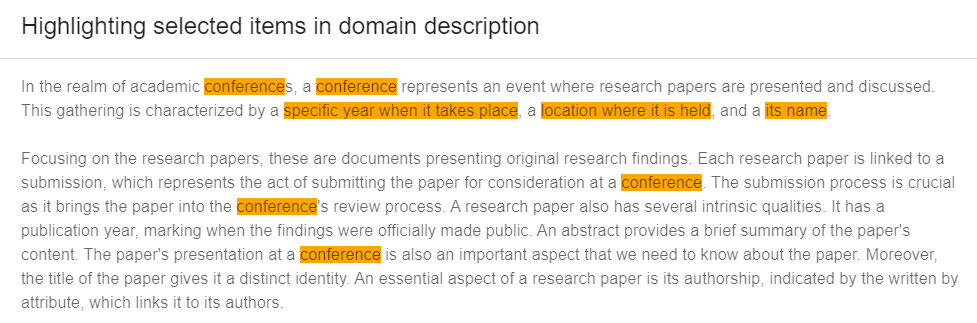
\includegraphics[scale=0.56]{../docs/images/frontend/highlight-all-example.png}
    \caption{\centering Example of highlighted original text in the domain description for the selected domain elements}
    \label{fig:highlight_all_example}
\end{figure}


For example, this feature can be used to check whether the domain model is completely representing the given domain description however, note that the assistant can make mistakes and that some part of the domain description is highlighted does not necessarily mean that it is represented by the domain model. Also, the opposite thing applies: some non-highlighted parts of the domain description can already be represented by the domain model.

For simplicity, whenever the domain description changes the computed original text indexes are discarded so nothing will be highlighted this means that for using this feature it is necessary to work with only one domain description without editing it in the process.


\section{Settings}

\begin{figure}[!h]
    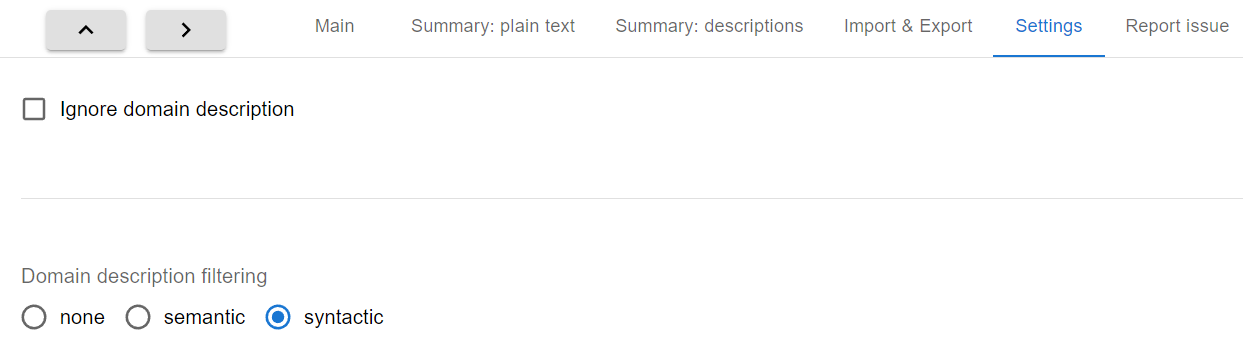
\includegraphics[scale=0.46]{../docs/images/frontend/settings.png}
    \caption{\centering Example of highlighted original text in the domain description for the selected domain elements}
    \label{fig:settings_tab}
\end{figure}

Figure \ref{fig:settings_tab} shows the settings tab. It contains an option to let the assistant ignore the domain description. Underneath the style of the summary plain text can be changed as discussed in the section \ref{sec:summarising_domain_model} and last but not least, the RAG strategy can be changed.


\section{Import and export}

In our repository\footnote{\url{https://github.com/Dominik7131/Conceptual-Modeling-LLM-Assistant/blob/master/docs/frontend-import-export.md}} there is also user documentation for importing and exporting a domain model both locally and with the Dataspecer tool\footnote{\url{https://dataspecer.com/}}.


\section{Demos}

Finally, in our repository\footnote{\url{https://github.com/Dominik7131/Conceptual-Modeling-LLM-Assistant/blob/master/docs/frontend-user.md\#demos}} are also links for videos demonstrating the work with our application.